\documentclass[11pt]{report}

%to add links but not color
\usepackage{hyperref}
%%Non-ASCII characters
\usepackage[utf8]{inputenc}

%LANGUAGES
\usepackage[english]{babel}

% Add draft watermark
\usepackage{draftwatermark}
\SetWatermarkScale{3}

%To add frames to verbatim environment
\usepackage{fancyvrb}

\topmargin=-1in    % Make letterhead start about 1 inch from top of page
\textheight=9in  % text height can be bigger for a longer letter
\oddsidemargin=0pt % leftmargin is 1 inch
\textwidth=6.5in   % textwidth of 6.5in leaves 1 inch for right margin
%%\usepackage[hyphens]{url}

%Bib style
\usepackage{natbib}
\bibpunct[: ]{(}{)}{;}{a}{,}{,}

%To Add Figures
\usepackage{graphicx}

\begin{document}
\title{Especificaciones para la anotación de SPinTX\\ con información lingüística para fines pedagógicos}
\author{Martí Quixal}
\date{Diciembre 2012 -- hoy}
\maketitle
\tableofcontents

\chapter*{Introducción}
Este documento describe el proceso de anotación de las transcripciones de los clips del corpus SPinTX (Spanish in Texas) con información pedagógica para facilitar el uso de los mismos en la enseñanza y el aprendizaje de español como lengua extranjera.

DOCU 
\part{Definición de LIST y SET}
\chapter{LIST y SET basados en información morfosintáctica}
\section{Categorías gramaticales}
\section{Rasgos morfosintácticos}
\chapter{LIST y SET basados en lemas}
\section{Los LIST}
\section{Los SET}
\chapter{LIST y SET basados en palabras (literales)}
\chapter{LIST y SET basados en etiquetas pedagógicas}
\part{Secciones previas}
\chapter{Reglas para rectificar errores del análisis morfosintático}
\begin{itemize}
\item ETIQ: CC
\item EJEM: \emph{pero} 
\item DESC: Regla para cambiar a \emph{pero} la lectura de nombre por la de conjunción. Ahora se aplica indiscriminadamente, pero podría ser conveniente controlar que antes del pero no hay un artículo. Por ejemplo: ``el pero de la cuestión es que podría romperse el motor''.
\end{itemize}

\begin{itemize}
\item ETIQ: Cambia Noun NC Singular Masculine por Verb VLadj
\item EJEM: \emph{hecho} 
\item DESC: Regla para cambiar a \emph{pero} la lectura de nombre por la de conjunción. Ahora se aplica indiscriminadamente, pero podría ser conveniente controlar que antes del pero no hay un artículo. Por ejemplo: ``el pero de la cuestión es que podría romperse el motor''.
\end{itemize}

\begin{itemize}
\item ETIQ: Cambia Verb VLfin Pres Indi Sing 1st por Noun NC Singular Masculine en la palabra ``rancho''.
\item EJEM: \emph{rancho} 
\item DESC: Lo hace de forma indiscriminada. Quizá en el futuro habrá que cambiarla, refinarla.
\end{itemize}

\begin{itemize}
\item ETIQ: Cambia lectura de ``dicho'' como determinante por lectura como adjetivo/participio.
\item EJEM: \emph{dicho} 
\item DESC: Lo hace de forma indiscriminada. Quizá en el futuro habrá que cambiarla, refinarla.
\end{itemize}

\begin{itemize}
\item ETIQ: Cambia lectura de "oye" como presente de subjuntivo por lectura de presente de indicativo/imperativo.
\item EJEM: \emph{oye} 
\item DESC: Lo hace de forma indiscriminada. Quizá en el futuro habrá que cambiarla, refinarla.
\end{itemize}

\begin{itemize}
\item ETIQ: Reglas que cambian la lectura de "ser" por "ir" en "fueron" cuando no va precedida de un pronombre se o seguida la preposición con o un gerundio.
\item EJEM: \emph{se fueron juntos, se fueron a la escuela} 
\item DESC: Quizá en el futuro habrá que cambiarlas, refinarlas.
\end{itemize}

\begin{itemize}
\item ETIQ: Cambia lectura de "maestro" de adjetivo sustantivo.
\item EJEM: \emph{maestro, maestra, maestros, maestras} 
\item DESC: Lo hace de forma indiscriminada. Quizá en el futuro habrá que cambiarla, refinarla. Por ejemplo, en "obras maestras", que no ocurre en la versión actal del corpus.
\end{itemize}

\begin{itemize}
\item ETIQ: Cambia lectura de "eras" y "eran" de lema ambiguo entre erar y ser a sólo lema ser.
\item EJEM: \emph{eras, eran} 
\item DESC: Consideramos erar un verbo muy poco frecuente. Si hiciera falta, se podría refinar la regla.
\end{itemize}

\part{Secciones principales}
Las reglas de identificación de fenómenmos pedagógicos están ordenadas de más concretas a más generales. Así, por ejemplo, se detectan primero, cuando es posible, los distintos usos de \emph{para} (opinión, intención, destino, etc. como \emph{@Gram:Prep:Para:Opinion}...) y luego se marcan como simplemente \emph{@Gram:Prep:Para} el resto de ocurrencias de \emph{para}. Luego, se hace lo propio con otras preposiciones, hasta el punto que si para una preposición no hay reglas especiales, sus ocurrencias se marcan simplemente como \emph{@Gram:Prep}.

Esta estrategia se utiliza para evitar que una misma palabra reciba por partida doble informaciones de igual granularidad. Para ello, antes de asignar una etiqueta, se comprueba que no haya otra asignada del mismo nivel. A efectos prácticos, etiquetas como \emph{@Gram:Prep:Para:Opinion}...) y \emph{@Gram:Prep:Para} se consideran del mismo nivel.

Para evitar este tipo de duplicidades también se podría usar una estrategia basada en la distinción entre ADD y MAP (véase la documentación de vislcg3). Por ahora no se ha hecho, porque esto impide la asignación de múltiples etiquetas a un mismo token/una misma palabra.

NOTA: Ahora mismo sólo estamos asignando hasta tres niveles de descripción pedagógica. Veáse el Google Doc Pedagogical tipologies \url{https://docs.google.com/spreadsheet/ccc?key=0AlyBsKogCRnwdDd3ZWRjejZlQU5XZWl6WVVUZmtKcEE&usp=sharing}.

\chapter{Uso de los determinantes}
\section{Usos de los artículos definidos}
Identificaremos los usos de los artículos definidos \emph{el, la, los, las}, y el artículo (en algunas gramáticas considerado pronombre) \emph{lo} cuando va seguido de un adjetivo.

\paragraph*{Rule}
\fbox{
\parbox{.9\linewidth}{\texttt{ADD (@Gram:Det:Art) Articulo IF (0 DetArtDefinidosLiterales) (NOT 1 FiniteVerbForms OR PronombreDeObjetoNoAmbiguos OR SeLiteral);}}
}
\begin{itemize}
\item ETIQ: Asigna @Gram:Det:Art
\item EJEM: \emph{el, la, los, las}
\item DESC: Cualquier ocurrencia no seguida de un verbo finito o un pronombre clítico, porque treetagger no distingue entre su lectura como determinante y la pronominal.
\end{itemize}

\paragraph*{Rule}
\fbox{
\parbox{.9\linewidth}{\texttt{ADD (@Gram:Det:Art) Articulo IF (0 LoLiteral) (*1 Adj BARRIER FiniteVerbForms OR Conjuncion OR LimiteOracionSimple) ;}}
}
\begin{itemize}
\item ETIQ: Asigna @Gram:Det:Art
\item EJEM: \emph{lo} + ADJETIVO
\item DESC: Cualquier ocurrencia de LO seguida de un adjetivo (con un adv opcional en medio).
\end{itemize}

\section{Usos de los determinantes demostrativos}
\paragraph*{Rule}
\fbox{
\parbox{.9\linewidth}{\texttt{ADD (@Gram:Det:Demo) ArtPronDemo IF (-1 Prep OR FiniteVerbForms) (0 EsteEseAquel) (NOT 0 EstoEsoAquello) (1 Nombre) ;}}
}
\begin{itemize}
\item ETIQ: Asigna @Gram:Det:Demo
\item EJEM: Prep/Verbo \emph{este/ese/aquel} (LEMMA) + Nombre
\item DESC: Cualquier ocurrencia de un demostrativo precedida de una preposición o un verbo conjugado y seguido de un nombre.
\end{itemize}

\section{Usos de los determinantes posesivos}
\paragraph*{Rule}
\fbox{
\parbox{.9\linewidth}{\texttt{ADD (@Gram:Det:Pos) DetPosSing IF (*1 Nombre + SG BARRIER FiniteVerbForms OR Conjuncion OR LimiteOracionSimple) ;}}
}
\paragraph*{Rule}
\fbox{
\parbox{.9\linewidth}{\texttt{ADD (@Gram:Det:Pos) DetPosPlu IF (*1 Nombre + PL BARRIER FiniteVerbForms OR Conjuncion OR LimiteOracionSimple) ;}}
}
\paragraph*{Rule}
\fbox{
\parbox{.9\linewidth}{\texttt{ADD (@Gram:Det:Pos) DetPosFemPlu IF (*1 Nombre + PL BARRIER FiniteVerbForms OR Conjuncion OR LimiteOracionSimple) ;}}
}
\paragraph*{Rule}
\fbox{
\parbox{.9\linewidth}{\texttt{ADD (@Gram:Det:Pos) DetPosMascPlu IF (*1 Nombre + PL BARRIER FiniteVerbForms OR Conjuncion OR LimiteOracionSimple) ;}}
}
\paragraph*{Rule}
\fbox{
\parbox{.9\linewidth}{\texttt{ADD (@Gram:Det:Pos) DetPosFemSing IF (*1 Nombre + SG BARRIER FiniteVerbForms OR Conjuncion OR LimiteOracionSimple) ;}}
}
\paragraph*{Rule}
\fbox{
\parbox{.9\linewidth}{\texttt{ADD (@Gram:Det:Pos) DetPosMascSing IF (*1 Nombre + SG BARRIER FiniteVerbForms OR Conjuncion OR LimiteOracionSimple) ;}}
}
\begin{itemize}
\item ETIQ: Asigna @Gram:Det:Poss
\item EJEM: Prep/Verbo \emph{mi/tu/su/sus/nuestro/nuestros/vuestro/vuestros} (LEMMA) + Nombre
\item DESC: Cualquier ocurrencia de un determinante posesivo seguido de un nombre (se admiten ADV y ADJ intercalados).
\end{itemize}

\chapter{Género gramatical y artículos}
\section{Género masculino en palabras terminadas en ``a''}
\paragraph*{Rule}
\fbox{
\parbox{.9\linewidth}{\texttt{ADDRELATION (Gram:Genero:ExcepMasc) DetAll IF (0 ElDetLiteral + SG OR UnDetLiteral + SG OR ArtPronDemo + SG) TO (1 SustMascAcabadosEnA + Nombre + SG) ;}}
}
\begin{itemize}
\item ETIQ: Asigna R:Gram:Genero:ExcepMasc
\item EJEM: \emph{el/un/ese} + (SUST acabado en -a, \emph{tema, día, problema, trauma})
\item DESC: No se aplica con todos los determinantes porque TreeTagger no asigna género a todos y lematiza con criterios curiosos.
\end{itemize}

\section{Cambio de artículo femenino a masculina en palabras con a tónica inicial}
\paragraph*{Rule}
\fbox{
\parbox{.9\linewidth}{\texttt{ADDRELATION (Gram:Genero:ExcepArtFem) DetAll IF (0 ElDetLiteral) TO (1 SustFemConATonicaInicial + Nombre + SG) ;}}
}
\begin{itemize}
\item ETIQ: Asigna R:Gram:Genero:ExcepArtFem
\item EJEM: \emph{el} + (SUST con a- tónica inicial, \emph{arma, aula, agua})
\item DESC: No se aplica con todos los determinantes porque TreeTagger no asigna género a todos y lematiza con criterios curiosos.
\end{itemize}

\chapter{Uso de las preposiciones}
\section{Usos de para}
Veáse \url{http://dev.coerll.utexas.edu/spanishtx/spe/html/adv11.html}.

\subsection{El uso de \emph{para} para expresar el destinatario o audiencia de una acción}
\paragraph*{Rule}
\fbox{
\parbox{.9\linewidth}{\texttt{ADD (@Gram:Prep:Para) Prep IF (-1 SerOServir + Verbo) (0 Para) (NOT 0 GramPrep) (1 DetAll) (2 Personas);}}
}
\begin{itemize}
\item ETIQ: Asigna @Gram:Prep:Para
\item EJEM: Fue escrito \emph{para} los estudiantes.
\item EJEM: Es fundamental \emph{para} una persona.
\item DESC: Requiere \emph{para + DET + NOMBRE $<+humano>$}
\end{itemize}

\paragraph*{Rule}
\fbox{
\parbox{.9\linewidth}{\texttt{ADD (@Gram:Prep:Para) Prep IF (-1 SerOServir + Verbo) (0 Para) (NOT 0 GramPrep) (1 Personas);}}
}
\begin{itemize}
\item ETIQ: Asigna @Gram:Prep:Para.
\item EJEM: Ropa \emph{para} niños.
\item DESC: Requiere \emph{para + NOMBRE $<+humano>$}
\end{itemize}

\subsection{El uso de \emph{para} para expresar una finalidad}
OBSERVACIÓN: Dudo de si el uso de ``Juan es muy bueno para el fútbol'' se parece o no al de ``hemos venido antes para no quedarnos sin asiento''. De momento los pongo juntos.

\paragraph*{Rule}
\fbox{
\parbox{.9\linewidth}{\texttt{ADD (@Gram:Prep:Para) Prep IF (0 Para) (NOT 0 GramPrep) (1 Infinitive);}}
}
\begin{itemize}
\item ETIQ: Asigna @Gram:Prep:Para.
\item EJEM: Soy muy mala \emph{para} recordar.
\item DESC: Requiere \emph{para + INFINITIVO}
\end{itemize}

\paragraph*{Rule}
\fbox{
\parbox{.9\linewidth}{\texttt{ADD (@Gram:Prep:Para) Prep IF (0 Para) (NOT 0 GramPrep) (1 PronPersFuerte OR No) (2 Infinitive);}}
}
\begin{itemize}
\item ETIQ: Asigna @Gram:Prep:Para.
\item EJEM: Había que saber hablar inglés \emph{para} uno desarrollar su trabajo.
\item DESC: Requiere \emph{para + PRONOMBRE PERSONAL NOMINATIVO + INFINITIVO}
\end{itemize}

\paragraph*{Rule}
\fbox{
\parbox{.9\linewidth}{\texttt{ADD (@Gram:Prep:Para) Prep IF (0 Para) (NOT 0 GramPrep) (1 Que);}}
}
\begin{itemize}
\item ETIQ: Asigna @Gram:Prep:Para.
\item EJEM: Me daba clases \emph{para} que aprendiera inglés.
\item DESC: Requiere \emph{para + QUE}
\end{itemize}

\subsection{El uso de \emph{para} para expresar una opinión}
\paragraph*{Rule}
\fbox{
\parbox{.9\linewidth}{\texttt{ADD (@Gram:Prep:Para) Prep IF (0 Para) (NOT 0 GramPrep) (1 PronombrePersonal) (NOT 1 YoLiteral OR TuLiteral);}}
}
\begin{itemize}
\item ETIQ: Asigna @Gram:Prep:Para.
\item EJEM: \emph{Para} mi.
\item DESC: Requiere \emph{para + PRONOMBRE PERSONAL ACUSATIVO}
\end{itemize}

 C: Esta regla es muy floja. Habrá que revisarla.
\subsection{Usos de \emph{para} no clasificados}
\paragraph*{Rule}
\fbox{
\parbox{.9\linewidth}{\texttt{ADD (@Gram:Prep:Para) Prep IF (0 Para) (NOT 0 GramPrep);}}
}
\begin{itemize}
\item ETIQ: Asigna @Gram:Prep:Para.
\item EJEM: \emph{para} (cualquier otra ocurrencia)
\item DESC: Requiere \emph{para}
\end{itemize}

\section{Usos de \emph{por}}
Veáse \url{http://dev.coerll.utexas.edu/spanishtx/spe/html/adv11.html}.

\subsection{Usos de \emph{por} en locuciones}
\paragraph*{Rule}
\fbox{
\parbox{.9\linewidth}{\texttt{ADD (@Gram:Prep:Por) Prep IF (0 Por) (NOT 0 GramPrep) (1 LemasDePalabrasEnLocucionesConPor OR FormasDePalabrasEnLocucionesConPor);}}
}
\begin{itemize}
\item ETIQ: Asigna @Gram:Prep:Por
\item EJEM: \emph{por ejemplo}, \emph{por eso}, \emph{por tanto}
\item DESC: Requiere \emph{por} seguida por alguna palabra en la lista de palabras predefinidas \emph{LemasDePalabrasEnLocucionesConPor}
\end{itemize}

\paragraph*{Rule}
\fbox{
\parbox{.9\linewidth}{\texttt{ADD (@Gram:Prep:Por) Prep IF (0 Por) (NOT 0 GramPrep) (1 LoLiteral) (2 LemasDePalabrasEnLocucionesConPor);}}
}
\begin{itemize}
\item ETIQ: Asigna @Gram:Prep:Por.
\item EJEM: \emph{por lo tanto}, \emph{por lo regular}
\item DESC: Requiere \emph{por} seguida por LO y alguna palabra en la lista de palabras predefinidas \emph{LemasDePalabrasEnLocucionesConPor}
\end{itemize}

\subsection{Usos de \emph{por} no clasificados}
\paragraph*{Rule}
\fbox{
\parbox{.9\linewidth}{\texttt{ADD (@Gram:Prep:Por) Prep IF (0 Por) (NOT 0 GramPrep);}}
}
\begin{itemize}
\item ETIQ: Asigna @Gram:Prep:Por.
\item EJEM: \emph{por} (cualquier ocurrencia)
\item DESC: Requiere \emph{por}
\end{itemize}

\subsection{Usos de preposiciones no clasificados}
\paragraph*{Rule}
\fbox{
\parbox{.9\linewidth}{\texttt{ADD (@Gram:Prep) Prep (NOT 0 GramPrep);}}
}
\begin{itemize}
\item ETIQ: Asigna @Gram:Prep.
\item EJEM: \emph{PREP} (cualquier ocurrencia)
\item DESC: Requiere \emph{PREP}
\end{itemize}

\chapter{Uso de los pronombres}
\section{Pronombres de sujeto}
\paragraph*{Rule}
\fbox{
\parbox{.9\linewidth}{\texttt{ADD (@Gram:Pron:Sujeto) PronPersFuerte;}}
}
\begin{itemize}
\item ETIQ: Asigna @Gram:Pron:Sujeto.
\item EJEM: \emph{yo, tú, él, ella, ud., nosotros, vosotros, ellos, ellas, uds.} (cualquier ocurrencia)
\item DESC: La ocurrencia de uno de ellos
\end{itemize}

\section{Pronombres de objeto directo o complemento atributivo}
\paragraph*{Rule}
\fbox{
\parbox{.9\linewidth}{\texttt{ADD (@Gram:Pron:Objeto) ElLema IF (NOT -1 Prep) (0 Articulo) (1 FiniteVerbForms) ;}}
}
\begin{itemize}
\item ETIQ: Asigna @Gram:Pron:Objeto
\item EJEM: mí nunca me \emph{la} hicieron pero que estabamos
\item DESC: \emph{lo, la, los, las} VERBO CONJUGADO
\end{itemize}

\section{Pronombres de objeto directo, indirecto, o posesivos}
\paragraph*{Rule}
\fbox{
\parbox{.9\linewidth}{\texttt{ADD (@Gram:Pron:Objeto) PronPers IF (0 PronombreDeObjetoNoAmbiguos);}}
}
\begin{itemize}
\item ETIQ: Asigna @Gram:Pron:Objeto
\item EJEM: \emph{me, te, os, nos} (cualquier ocurrencia)
\item DESC: La ocurrencia de uno de ellos.
\end{itemize}

\section{Pronombres de objeto indirecto}
\paragraph*{Rule}
\fbox{
\parbox{.9\linewidth}{\texttt{ADD (@Gram:Pron:Objeto) PronPersClitico IF (0 LeLema);}}
}
\begin{itemize}
\item ETIQ: Asigna @Gram:Pron:Objeto
\item EJEM: \emph{le, les}
\item DESC: La ocurrencia de uno de ellos.
\end{itemize}

\section{Pronombres de objeto doble}
\paragraph*{Rule}
\fbox{
\parbox{.9\linewidth}{\texttt{ADDRELATION (Gram:Pron:ObjetoDoble) PronPers (0 PronombreDeObjetoNoAmbiguos) TO (1 ElLema + Articulo);}}
}
\paragraph*{Rule}
\fbox{
\parbox{.9\linewidth}{\texttt{ADDRELATION (Gram:Pron:ObjetoDoble) PronPersSE (0 SeLiteral) TO (1 ElLema + Articulo);}}
}
\begin{itemize}
\item ETIQ: Asigna @Gram:Pron:ObjetoDoble.
\item EJEM: \emph{se lo, se la, se los, se las, me lo, me la, me los, me las, te lo, te la, te los, te las,} etc.
\item DESC: La ocurrencia de cualquier combinación de dos pronombres clíticos.
\end{itemize}

\section{Pronombre se (solo)}
\paragraph*{Rule}
\fbox{
\parbox{.9\linewidth}{\texttt{ADD (@Gram:Pron:Otros) PronPersSE (0 SeLiteral) (NOT 0 GramPron) (NOT 1 FiniteVerbForms);}}
}
\begin{itemize}
\item ETIQ: Asigna @Gram:Pron:Otros.
\item EJEM: \emph{se lo, se la, se los, se las, me lo, me la, me los, me las, te lo, te la, te los, te las,} etc.
\item DESC: La ocurrencia de cualquier combinación de dos pronombres clíticos.
\end{itemize}

\chapter{Formas verbales conjugadas}
\section{Formas verbales para tiempos de indicativo}
\subsection{Pretérito imperfecto}
\paragraph*{Rule}
\fbox{
\parbox{.9\linewidth}{\texttt{ADD (@Gram:Imperf) FiniteVerbForms IF (0 FiniteVerbForms + PretImperfSimple) (NOT 0 Haber) ;}}
}
\begin{itemize}
\item ETIQ: Asigna @Gram:Imperf.
\item EJEM: \emph{cantaba, corría, temía, partía} (cualquier ocurrencia)
\item DESC: Requiere una forma identificada como pretérito simple que no sea del verbo haber (auxiliar).
\end{itemize}

\subsection{Pretérito perfecto}
\subsubsection{Pretérito perfecto simple}
\paragraph*{Rule}
\fbox{
\parbox{.9\linewidth}{\texttt{ADD (@Gram:Indefinido) FiniteVerbForms IF (0 FiniteVerbForms + PretPerfSimple) (NOT 0 Haber) ;}}
}
\begin{itemize}
\item ETIQ: Asigna @Gram:PretPerf.
\item EJEM: \emph{cantó, corrió, anduvo, partió} (cualquier ocurrencia)
\item DESC: Requiere una forma identificada como pretérito perfecto simple que no sea del verbo haber (auxiliar).
\end{itemize}

\subsubsection{Pretérito perfecto perifrástico o compuesto}\label{sec:HaberAuxPretPerfecto}
\paragraph*{Rule}
\fbox{
\parbox{.9\linewidth}{\texttt{ADDRELATION (Gram:PerfPerif Gram:Aux:Haber) FiniteVerbForms (0 Haber + FiniteVerbForms + Presente) (NOT 0 Subjuntivo) TO (1 Part);}}
}
\begin{itemize}
\item ETIQ: Asigna R:Gram:PerfPerif a la forma del verbo HABER
\item EJEM: \emph{ha cantado, ha corrido, ha andado dormido} (cualquier ocurrencia)
\item DESC: Requiere una forma finita de HABER seguida de un participio
\end{itemize}

\section{Verbos piscológicos: gustar, encantar, sorprender y otros}
Veáse \url{http://dev.coerll.utexas.edu/spanishtx/spe/html/adv13.html}.

Veáse \url{http://dev.coerll.utexas.edu/spanishtx/spe/html/beg05.html}.

\subsection{Usos de \emph{gustar} para expresar gustos propios}
\paragraph*{Rule}
\fbox{
\parbox{.9\linewidth}{\texttt{ADDRELATION (Gram:Gustar:Propios) PronPers (0 Me OR NosLiteral) TO (1 Gustar-Like + 3aPersAmbig);}}
}
\begin{itemize}
\item ETIQ: Asigna @Gram:Gustar:Propios.
\item EJEM: \emph{me gusta} ayudar a mis amigos 
\item DESC: Requiere la forma ME seguida de una forma de GUSTAR en tercera persona (posiblemente ambigua)
\end{itemize}

\paragraph*{Rule}
\fbox{
\parbox{.9\linewidth}{\texttt{ADDRELATION (Gram:Gustar:Propios) PronPers (0 Me OR NosLiteral) (1 Haber) TO (1 Gustar-Like + Part);}}
}
\begin{itemize}
\item ETIQ: Asigna R:Gram:Gustar: Propios a la forma del verbo HABER
\item EJEM: \emph{me ha gustado} ayudar a mis amigos 
\item EJEM: \emph{me hubieras gustado} con un vestido verde 
\item DESC: Requiere la forma ME seguida de una forma de HABER en tercera persona (posiblemente ambigua)
\end{itemize}

\subsection{Usos de \emph{gustar} para expresar gustos de tu interlocutor}
\paragraph*{Rule}
\fbox{
\parbox{.9\linewidth}{\texttt{ADD (@Gram:Gustar:Interlocutor) FiniteVerbForms IF  (-1 Tu) (0 Gustar-Like + 3aPersAmbig);}}
}
\begin{itemize}
\item ETIQ: @Gram:Gustar:Interlocutor
\item EJEM: Dime, \emph{te gusta} vivir en Estados Unidos.] 
\item DESC: Secuencia del lema TE y un forma de GUSTAR en tercera persona del singular.
\end{itemize}

\subsection{Usos de \emph{gustar} para expresar gustos de otras personas}
\paragraph*{Rule}
\fbox{
\parbox{.9\linewidth}{\texttt{ADDRELATION (Gram:Gustar:Ajenos) FiniteVerbForms (0 Gustar-Like + 3aPersAmbig) TO (-1 LeLema);}}
}
\begin{itemize}
\item ETIQ: R:Gram:Gustar:Ajenos a la forma del verbo GUSTAR
\item EJEM: Dime, \emph{le gusta} vivir en Estados Unidosa tu hijo.] 
\item DESC: Secuencia del lema LE y un forma de GUSTAR en tercera persona del singular.
\end{itemize}

\section{Expresar sorpresa}
Veáse \url{http://dev.coerll.utexas.edu/spanishtx/spe/html/adv13.html}.

\subsection{Usos de \emph{sorprender}}
\paragraph*{Rule}
\fbox{
\parbox{.9\linewidth}{\texttt{ADDRELATION (Gram:Gustar:Otros) FiniteVerbForms (0 Sorprender-Like + 3aPersAmbig) TO (-1 Yo);}}
}
\begin{itemize}
\item ETIQ: Asigna Gram:Gustar:Otros (Gram:ExpresarSorpresas:Propias) a la forma de SORPRENDER
\item EJEM: Siempre \emph{me sorprende} su forma de hablar.
\item DESC: [Espacio para describir con palabras lo que hace la regla.]
\end{itemize}

\paragraph*{Rule}
\fbox{
\parbox{.9\linewidth}{\texttt{ADDRELATION (Gram:Gustar:Otros) FiniteVerbForms (0 Sorprender-Like + 3aPersAmbig) TO (-1 Tu);}}
}
\begin{itemize}
\item ETIQ: Asigna Gram:Gustar:Otros (antes era Gram:ExpresarSorpresas:Interlocutor) a la forma de SORPRENDER
\item EJEM: ¿Y \emph{te sorprende} su forma de hablar?
\item DESC: [Espacio para describir con palabras lo que hace la regla.]
\end{itemize}

\paragraph*{Rule}
\fbox{
\parbox{.9\linewidth}{\texttt{ADDRELATION (Gram:Gustar:Otros) Part (0 Sorprender-Like) TO (*-1 Tu BARRIER GrupoNominal OR LimiteOracionSimple LINK 1 Haber + 3aPersAmbig);}}
}
\begin{itemize}
\item ETIQ: Asigna Gram:Gustar:Otros (antes era Gram:ExpresarSorpresas:Interlocutor) a la forma de HABER
\item EJEM: ¿Hay alguna palabra mexicana que \emph{te haya sorprendido}?
\item DESC: [Espacio para describir con palabras lo que hace la regla.]
\end{itemize}

\paragraph*{Rule}
\fbox{
\parbox{.9\linewidth}{\texttt{ADDRELATION (Gram:Gustar:Otros) FiniteVerbForms (0 Sorprender-Like + 3aPersAmbig) TO (-1 LeLema);}}
}
\begin{itemize}
\item ETIQ: Asigna Gram:Gustar:Otros (antes era Gram:ExpresarSorpresas:Ajenas) a la forma de SORPRENDER
\item EJEM: ¿Y \emph{le sorprende} su forma de hablar?
\item DESC: [Espacio para describir con palabras lo que hace la regla.]
\end{itemize}

\paragraph*{Rule}
\fbox{
\parbox{.9\linewidth}{\texttt{ADDRELATION (Gram:Gustar:Otros) Part (0 Sorprender-Like) TO (*-1 LeLema BARRIER GrupoNominal OR LimiteOracionSimple LINK 1 Haber + 3aPersAmbig);}}
}
\begin{itemize}
\item ETIQ: Asigna Gram:Gustar:Otros (antes era Gram:ExpresarSorpresas:Ajenas) a la forma de HABER
\item EJEM: ¿Hay alguna palabra mexicana que \emph{le haya sorprendido}?
\item DESC: [Espacio para describir con palabras lo que hace la regla.]
\end{itemize}

\section{Formas verbales para tiempos de subjuntivo}
\paragraph*{Rule}
\fbox{
\parbox{.9\linewidth}{\texttt{ADD (@Gram:MSub:Pres) Verbo IF (0 Presente + Subjuntivo) (NOT -1 De) (NOT 1 Part);}}
}
\paragraph*{Rule}
\fbox{
\parbox{.9\linewidth}{\texttt{ADD (@Gram:MSub:Pret) FiniteVerbForms IF (0 Verbo + Pasado + Subjuntivo) (NOT -1 De) (NOT 1 Part);}}
}
\paragraph*{Rule}
\fbox{
\parbox{.9\linewidth}{\texttt{ADDRELATION (Gram:MSub:Pres) FiniteVerbForms (0 Haber + Verbo + Presente + Subjuntivo) (NOT -1 De) TO (1 Part);}}
}
\paragraph*{Rule}
\fbox{
\parbox{.9\linewidth}{\texttt{ADDRELATION (Gram:MSub:Pret) FiniteVerbForms (0 Haber + Verbo + Pasado + Subjuntivo) (NOT -1 De) TO (1 Part);}}
}
\begin{itemize}
\item ETIQ: Asigna Gram:MSub:Pres a verbos en presente o pretérito de subjuntivo
\item EJEM: ¿Hay alguna palabra mexicana que \emph{le haya sorprendido}?
\item DESC: No se aplica si la forma verbal no esta precedida por una "de" para evitar formas incorrectamente marcadas como subjuntivo por el tagging básico. Si se trata de una forma compuesta, es decir, HABER + PART, se marca todo como tal.
\end{itemize}

\section{Verbos copulativos}
\subsection{Verbo ser}
\paragraph*{Rule}
\fbox{
\parbox{.9\linewidth}{\texttt{ADD (@Gram:SerEstar:Ser) Verbo (0 VerboSer OR VerboSerAmbiguoConErar) (NOT -1 Haber);}}
}
\paragraph*{Rule}
\fbox{
\parbox{.9\linewidth}{\texttt{ADD (@Gram:SerEstar:Ser) Verbo (0 VerboSerAmbiguoConIr) (NOT 1 Prep) (NOT -1 Haber);}}
}
\paragraph*{Rule}
\fbox{
\parbox{.9\linewidth}{\texttt{ADDRELATION (Gram:SerEstar:Ser) Verbo (0 Haber + FiniteVerbForms) TO (1 VerboSer + Part OR VerboSerAmbiguoConErar + Part) (NOT 1 Part);}}
}
\begin{itemize}
\item ETIQ: @Gram:SerEstar:Ser
\item EJEM: \emph{soy, eres,} \emph{ha sido,}, pero no \emph{ha sido comprado}etc. 
\item EJEM: \emph{fui, fuimos...} NOT Prep 
\item DESC: Cualquier forma de \emph{ser} del pretérito indefinido no seguido de una preposición (porque entonces seguramente será del verbo ir). También las formas perifrásticas con haber que no vayan seguidas de un participició
\end{itemize}

\subsection{Verbo estar}
\paragraph*{Rule}
\fbox{
\parbox{.9\linewidth}{\texttt{ADD (@Gram:SerEstar:Estar) Verbo (0 VerboEstar);}}
}
\begin{itemize}
\item ETIQ: @Gram:SerEstar:Estar
\item EJEM: \emph{estoy, estás, estaban,} etc. 
\item DESC: Cualquier forma de \emph{estar}
\end{itemize}

\section{Verbo haber}
\subsection{Verbo haber en su uso com existencial}
\paragraph*{Rule}
\fbox{
\parbox{.9\linewidth}{\texttt{ADD (@Gram:Haber:Exist) Verbo (0 Haber) (NOT 1 Part);}}
}
\begin{itemize}
\item ETIQ: @Gram:Haber:Exist
\item EJEM: \emph{Había} tres personas en el ascensor. 
\item DESC: Cualquier forma de \emph{haber} que no vaya seguida de un participio
\end{itemize}

\section{Verbos auxiliares: ser, estar y haber}
\subsection{Verbo estar en su uso como auxiliar}
Se etiqueta con RGram:SerEstar:EstarAux las secuencias de estar seguido de un gerundio.

\paragraph*{Rule}
\fbox{
\parbox{.9\linewidth}{\texttt{ADDRELATION (Gram:SerEstar:EstarAux) VerboEstar IF (0 FiniteVerbForms) TO (1 Gerundio);}}
}
\paragraph*{Rule}
\fbox{
\parbox{.9\linewidth}{\texttt{ADDRELATION (Gram:SerEstar:EstarAux) VerboEstar IF (0 Infinitive) TO (1 Gerundio);}}
}
\begin{itemize}
\item ETIQ: R:Gram:SerEstar:EstarAux
\item EJEM: y me \emph{estuvo platicando} allí
\item DESC: Actualmente sólo se aplica sobre formas conjugadas y en secuencias estar (infinitivo) más gerundio. Habrá que ver cuán necesario es aplicar reglas para "hemos estado mirando" o "estando comprando?" (el interrogante los uso para marcar que dudo de la gramaticalidad de esta oración.
\end{itemize}

\subsection{Verbo haber en su uso como auxiliar en tiempos verbales compuestos}
Se etiqueta con @Gram:Aux:Haber, pero se hace en las reglas que sirven para etiquetar los tiempos verbales correspondientes. Véase por ejemplo la anotación (y la regla) del Presente Perfecto en la sección \ref{sec:HaberAuxPretPerfecto}. 

\subsection{Verbo ser en su uso como auxiliar}
\begin{figure}[htb]

\centering

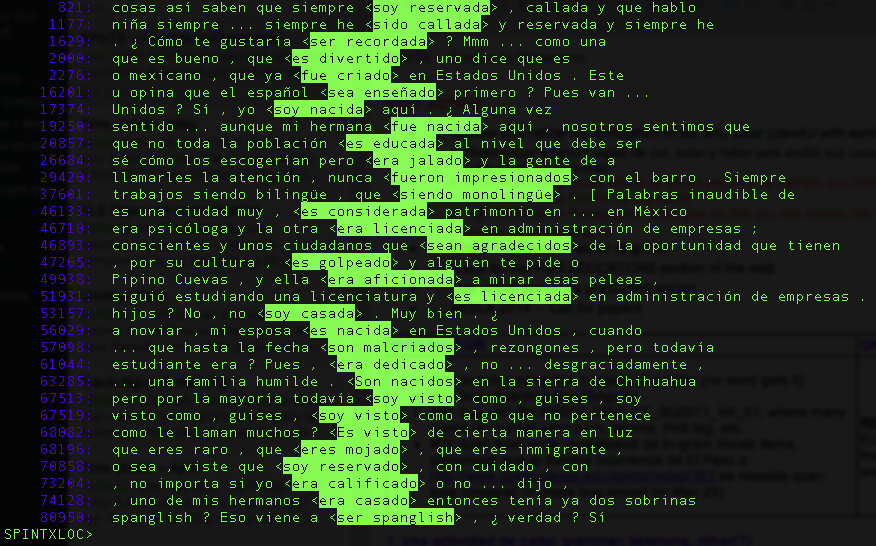
\includegraphics[scale=0.5]{Figs/InstancesOfSerPlusParticiple.png}

\caption{Ocurrencias de ser seguido de participio en Batch 1.}

\label{fig:InstancesOfSerPlusParticiple}

\end{figure}

\chapter{Funciones comunicativas}
\chapter{Pragmática}
\section{Marcadores discursivos}
Véase \url{http://www.cs.famaf.unc.edu.ar/~laura/shallowdisc4summ/index.html}.

\subsection{Marcadores discursivos indicadores de revisión}
\paragraph*{Rule}
\fbox{
\parbox{.9\linewidth}{\texttt{ADD (@Prag:MarcadoresDisc:Revision) MarcDiscRevision;}}
}
\begin{itemize}
\item ETIQ: @:Prag:MarcadoresDisc:Revision
\item EJEM: \emph{aunque}, \emph{excepto} o \emph{pero}
\item DESC: [Espacio para describir con palabras lo que hace la regla.]
\end{itemize}

\paragraph*{Rule}
\fbox{
\parbox{.9\linewidth}{\texttt{ADDRELATION (Prag:MarcadoresDisc:Revision) Sin TO (1 Embargo);}}
}
\begin{itemize}
\item ETIQ: R:Prag:MarcadoresDisc:Revision (relación entre el primer i el último elemento de la locución)
\item EJEM: \emph{sin embargo}
\item DESC: [Espacio para describir con palabras lo que hace la regla.]
\end{itemize}

\paragraph*{Rule}
\fbox{
\parbox{.9\linewidth}{\texttt{ADDRELATION (Prag:MarcadoresDisc:Revision) De TO (1 Hecho);}}
}
\begin{itemize}
\item ETIQ: R:Prag:MarcadoresDisc:Revision (relación entre el primer i el último elemento de la locución)
\item EJEM: \emph{de hecho}
\item DESC: [Espacio para describir con palabras lo que hace la regla.]
\end{itemize}

\paragraph*{Rule}
\fbox{
\parbox{.9\linewidth}{\texttt{ADDRELATION (Prag:MarcadoresDisc:Revision) En TO (1 Realidad);}}
}
\begin{itemize}
\item ETIQ: R:Prag:MarcadoresDisc:Revision (relación entre el primer i el último elemento de la locución)
\item EJEM: \emph{en realidad}
\item DESC: [Espacio para describir con palabras lo que hace la regla.]
\end{itemize}

\paragraph*{Rule}
\fbox{
\parbox{.9\linewidth}{\texttt{ADDRELATION (Prag:MarcadoresDisc:Revision) APrep (1 Pesar) TO (2 De);}}
}
\begin{itemize}
\item ETIQ: R:Prag:MarcadoresDisc:Revision (relación entre el primer i el último elemento de la locución)
\item EJEM: \emph{a pesar de}
\item DESC: [Espacio para describir con palabras lo que hace la regla.]
\end{itemize}

\paragraph*{Rule}
\fbox{
\parbox{.9\linewidth}{\texttt{ADDRELATION (Prag:MarcadoresDisc:Revision) De (1 Todos) TO (2 Modos);}}
}
\begin{itemize}
\item ETIQ: R:Prag:MarcadoresDisc:Revision (relación entre el primer i el último elemento de la locución)
\item EJEM: \emph{de todos modos}
\item DESC: [Espacio para describir con palabras lo que hace la regla.]
\end{itemize}

\paragraph*{Rule}
\fbox{
\parbox{.9\linewidth}{\texttt{ADDRELATION (Prag:MarcadoresDisc:Revision) Es (1 Cierto) TO (2 Que);}}
}
\begin{itemize}
\item ETIQ: R:Prag:MarcadoresDisc:Revision (relación entre el primer i el último elemento de la locución)
\item EJEM: \emph{s cierto que}
\item DESC: [Espacio para describir con palabras lo que hace la regla.]
\end{itemize}

\subsection{Marcadores discursivos indicadores de causa}
\paragraph*{Rule}
\fbox{
\parbox{.9\linewidth}{\texttt{ADD (@Prag:MarcadoresDisc:Causa) Porque;}}
}
\begin{itemize}
\item ETIQ: @Prag:MarcadoresDisc:Causa
\item DESC: [Espacio para describir con palabras lo que hace la regla.]
\end{itemize}

\paragraph*{Rule}
\fbox{
\parbox{.9\linewidth}{\texttt{ADDRELATION (Prag:MarcadoresDisc:Causa) Prep IF (0 Por) (1 LoLiteral) TO (2 Tanto);}}
}
\paragraph*{Rule}
\fbox{
\parbox{.9\linewidth}{\texttt{ADDRELATION (Prag:MarcadoresDisc:Causa) Prep IF (0 Por) TO (2 Tanto OR FormasDePalabrasEnLocucionesCausalesConPor);}}
}
\begin{itemize}
\item ETIQ: Asigna @Prag:MarcadoresDisc:Causa.
\item EJEM: \emph{por lo tanto}
\item EJEM: \emph{por eso}
\item DESC: Requiere \emph{por} seguida por LO y TANTO
\end{itemize}

\paragraph*{Rule}
\fbox{
\parbox{.9\linewidth}{\texttt{ADDRELATION (Prag:MarcadoresDisc:Causa) Debido TO (1 APrep);}}
}
\begin{itemize}
\item ETIQ: R:Prag:MarcadoresDisc:Causa (relación entre el primer i el último elemento de la locución)
\item DESC: [Espacio para describir con palabras lo que hace la regla.]
\end{itemize}

\paragraph*{Rule}
\fbox{
\parbox{.9\linewidth}{\texttt{ADDRELATION (Prag:MarcadoresDisc:Causa) Gracia (0 PL) (NOT 2 Dios) TO (1 APrep);}}
}
\begin{itemize}
\item ETIQ: R:Prag:MarcadoresDisc:Causa (relación entre el primer i el último elemento de la locución)
\item DESC: [Espacio para describir con palabras lo que hace la regla.]
\end{itemize}

\paragraph*{Rule}
\fbox{
\parbox{.9\linewidth}{\texttt{ADDRELATION (Prag:MarcadoresDisc:Causa) Gracia (0 PL) (1 APrep) TO (2 Dios);}}
}
\begin{itemize}
\item ETIQ: R:Prag:MarcadoresDisc:Causa (relación entre el primer i el último elemento de la locución)
\item EJEM: y de ahí fui a la ceremonia y \emph{gracias a dios} me hice ciudadano
\item DESC: [Espacio para describir con palabras lo que hace la regla.]
\end{itemize}

\subsection{Marcadores discursivos indicadores de igualdad}
\paragraph*{Rule}
\fbox{
\parbox{.9\linewidth}{\texttt{ADD (@Prag:MarcadoresDisc:Igualdad) Adv IF (0 Ademas) (NOT 1 De);}}
}
\paragraph*{Rule}
\fbox{
\parbox{.9\linewidth}{\texttt{ADD (@Prag:MarcadoresDisc:Igualdad) Adv IF (0 Tambien);}}
}
OBSERVACIÓN: No añado \emph{precisamente} porque es ambiguo entre su lectura literal (preciso, justo, cierto) como modificador verbal y su lectura como marcador discursivo. Para anotarlo con fiabilidad habría que tener en cuenta su posición respecto al principio de la oración y el verbo principal. Ejemplos: \emph{sí muchas pero no sé precisamente cuál cuál sería una}, \emph{allí vivimos como un año y precisamente yo me tomé me tomaron fotos en un un estudio de fotografía}

\begin{itemize}
\item ETIQ: @:Prag:MarcadoresDisc:Igualdad
\item EJEM: \emph{además}, \emph{también}
\item DESC: Requiere \emph{además} o \emph{también} no seguido de DE
\end{itemize}

\paragraph*{Rule}
\fbox{
\parbox{.9\linewidth}{\texttt{ADDRELATION (Prag:MarcadoresDisc:Igualdad) Prep IF (0 Por) TO (1 Ejemplo);}}
}
\begin{itemize}
\item ETIQ: R:Prag:MarcadoresDisc:Igualdad (relación entre el primer i el último elemento de la locución)
\item EJEM: \emph{por ejemplo}
\item DESC: Requiere \emph{por} seguida por alguna palabra en la lista de palabras predefinidas \emph{LemasDePalabrasEnLocucionesConPor}
\end{itemize}

\paragraph*{Rule}
\fbox{
\parbox{.9\linewidth}{\texttt{ADDRELATION (Prag:MarcadoresDisc:Igualdad) ConjLetraO TO (1 Sea);}}
}
\begin{itemize}
\item ETIQ: R:Prag:MarcadoresDisc:Igualdad
\item EJEM: \emph{o sea}
\item DESC: [Espacio para describir con palabras lo que hace la regla.]
\end{itemize}

\paragraph*{Rule}
\fbox{
\parbox{.9\linewidth}{\texttt{ADDRELATION (Prag:MarcadoresDisc:Igualdad) No TO (1 SoloAcento);}}
}
\begin{itemize}
\item ETIQ: R:Prag:MarcadoresDisc:Igualdad
\item EJEM: porque uno \emph{no sólo} puede ayudar en el aspecto de inglés pero en el aspecto del español también
\item DESC: [Espacio para describir con palabras lo que hace la regla.]
\end{itemize}

\paragraph*{Rule}
\fbox{
\parbox{.9\linewidth}{\texttt{ADDRELATION (Prag:MarcadoresDisc:Igualdad) Tal TO (1 Vez);}}
}
\begin{itemize}
\item ETIQ: R:Prag:MarcadoresDisc:NoTipificado
\item EJEM: noto que \emph{tal vez} sus hijos hablan el spanglish más unos más que otros
\item DESC: [Espacio para describir con palabras lo que hace la regla.]
\end{itemize}

\subsection{Elementos discursivos usadors para ganar tiempo}
\paragraph*{Rule}
\fbox{
\parbox{.9\linewidth}{\texttt{ADD (@Prag:RecuDiscurso:GanarTiempo) ArtPronDemo IF (NOT -1 Prep) (0 EsteLiteral) (NOT 1 Nombre);}}
}
\begin{itemize}
\item ETIQ: @Prag:ElementosDiscurso:GanarTiempo
\item EJEM: \emph{Este} en mi niñez era un poco más soñadora mucho más soñadora de hecho (...)
\item DESC: Anota ocurrencies de ESTE que no vayan precedidas de una preposición ni seguidas de un sustantivo.
\end{itemize}

\chapter{Estructuras características del habla en hablantes de herencia}
\section{Estructuras derivadas del contacto entre lenguas}
\subsection{Expresiones con cambio de código}
Incluímos aquí expresiones que mezclan palabras en ambas lenguas, en este caso el español y el inglés. En la bibliografía especializada se utiliza el término inglés ``code switching''.

\paragraph*{Rule}
\fbox{
\parbox{.9\linewidth}{\texttt{ADDRELATION (Herit:Contacto:Mixtas) Verbo IF (0 ListaVerbosCorpusParaContactoMixtos) TO (*1 PalabraEnIngles BARRIER PalabraEnEspanol);}}
}
\begin{itemize}
\item ETIQ: R:Herit:Contacto:Mixtas
\item EJEM: \emph{hacer request}, \emph{comer turkey}
\item DESC: Anota secuencias de un verbo seguid de una o más palabras en inglés. Por ahora lo limitamos a ser, hacer, decir y comer porque TreeTagger anota como verbo algunas palabras que no lo son y no queremos generar ruido para los usuarios.
\end{itemize}

\chapter{Vocabulario multipalabra}
\section{Nombres propios}
\subsection{Nombres de localizaciones geográficas}
\paragraph*{Rule}
\fbox{
\parbox{.9\linewidth}{\texttt{ADDRELATION (Vocab:Entities:Geo) Articulo IF  (0 ("<El>")) TO (1 ("<Paso>"));}}
}
\paragraph*{Rule}
\fbox{
\parbox{.9\linewidth}{\texttt{ADDRELATION (Vocab:Entities:Geo) Nombre IF  (0 ("<Estados>")) TO (1 ("<Unidos>"));}}
}
\paragraph*{Rule}
\fbox{
\parbox{.9\linewidth}{\texttt{ADDRELATION (Vocab:Entities:Geo) Nombre IF  (0 ("<Ciudad>")) TO (1 ("<Juárez>"));}}
}
\begin{itemize}
\item ETIQ: R:Vocab:Entities:Geo
\item EJEM: \emph{Ciudad Juárez}, \emph{El Paso}, \emph{Estados Unidos}  
\item DESC: Reglas para anotar entidades frecuentes en el corpus. En este caso de nombres geográficos.
\end{itemize}

\subsection{Combinaciones de verbo y preposición de régimen}
\paragraph*{Rule}
\fbox{
\parbox{.9\linewidth}{\texttt{ADDRELATION (Vocab:Fraseol:VerbPrep) Verbo IF  (0 ("hablar")) TO (*1 Prep BARRIER LimiteOracionSimple OR GrupoNominal OR Verbo);}}
}
\paragraph*{Rule}
\fbox{
\parbox{.9\linewidth}{\texttt{ADDRELATION (Vocab:Fraseol:VerbPrep) Verbo IF  (0 ("pensar")) TO (*1 Prep BARRIER LimiteOracionSimple OR GrupoNominal OR Verbo);}}
}
\paragraph*{Rule}
\fbox{
\parbox{.9\linewidth}{\texttt{ADDRELATION (Vocab:Fraseol:VerbPrep) Verbo IF  (0 ("empezar")) TO (*1 Prep BARRIER LimiteOracionSimple OR GrupoNominal OR Verbo);}}
}
\begin{itemize}
\item ETIQ: R:Vocab:Fraseol:VerbPrep
\item EJEM: \emph{hablar PREP}, \emph{pensar PREP}, \emph{empezar PREP}  
\item DESC: Ahora no se distingue entre usos lexicalizados y usos composicionales (p.e., ``empezar en San Antonio y terminar en Austin'' se trata igual que ``empezé con la tradición en la preparatoria'') 
\end{itemize}

\end{document}